\documentclass[11pt]{aghdpl}
% \documentclass[en,11pt]{aghdpl}  % praca w języku angielskim

% Lista wszystkich języków stanowiących języki pozycji bibliograficznych użytych w pracy.
% (Zgodnie z zasadami tworzenia bibliografii każda pozycja powinna zostać utworzona zgodnie z zasadami języka, w którym dana publikacja została napisana.)
\usepackage[english,polish]{babel}

% Użyj polskiego łamania wyrazów (zamiast domyślnego angielskiego).
\usepackage{polski}

\usepackage[utf8]{inputenc}

% dodatkowe pakiety

\usepackage{mathtools}
\usepackage{amsfonts}
\usepackage{amsmath}
\usepackage{amsthm}
\usepackage{graphicx}

% --- < bibliografia > ---

\usepackage[
style=numeric,
sorting=none,
%
% Zastosuj styl wpisu bibliograficznego właściwy językowi publikacji.
language=autobib,
autolang=other,
% Zapisuj datę dostępu do strony WWW w formacie RRRR-MM-DD.
urldate=iso8601,
% Nie dodawaj numerów stron, na których występuje cytowanie.
backref=false,
% Podawaj ISBN.
isbn=true,
% Nie podawaj URL-i, o ile nie jest to konieczne.
url=false,
%
% Ustawienia związane z polskimi normami dla bibliografii.
maxbibnames=3,
% Jeżeli używamy BibTeXa:
backend=bibtex
]{biblatex}

\usepackage{csquotes}
% Ponieważ `csquotes` nie posiada polskiego stylu, można skorzystać z mocno zbliżonego stylu chorwackiego.
\DeclareQuoteAlias{croatian}{polish}

\addbibresource{bibliografia}

% Nie wyświetlaj wybranych pól.
%\AtEveryBibitem{\clearfield{note}}


% ------------------------
% --- < listingi > ---

% Użyj czcionki kroju Courier.
\usepackage{courier}

\usepackage{listings}
\lstloadlanguages{TeX}

\lstset{
	literate={ą}{{\k{a}}}1
           {ć}{{\'c}}1
           {ę}{{\k{e}}}1
           {ó}{{\'o}}1
           {ń}{{\'n}}1
           {ł}{{\l{}}}1
           {ś}{{\'s}}1
           {ź}{{\'z}}1
           {ż}{{\.z}}1
           {Ą}{{\k{A}}}1
           {Ć}{{\'C}}1
           {Ę}{{\k{E}}}1
           {Ó}{{\'O}}1
           {Ń}{{\'N}}1
           {Ł}{{\L{}}}1
           {Ś}{{\'S}}1
           {Ź}{{\'Z}}1
           {Ż}{{\.Z}}1,
	basicstyle=\footnotesize\ttfamily,
}

% ------------------------

\AtBeginDocument{
	\renewcommand{\tablename}{Tabela}
	\renewcommand{\figurename}{Rys.}
}

% ------------------------
% --- < tabele > ---

\usepackage{array}
\usepackage{tabularx}
\usepackage{multirow}
\usepackage{booktabs}
\usepackage{makecell}

% defines the X column to use m (\parbox[c]) instead of p (`parbox[t]`)
\newcolumntype{C}[1]{>{\hsize=#1\hsize\centering\arraybackslash}X}


%---------------------------------------------------------------------------

\author{Szymon Szczęsny}
\shortauthor{Sz. Szczęsny}

\titlePL{Prototyp układu aktywnej redukcji poziomu hałasu}
\titleEN{Prototype of an active noise reduction system}

\shorttitlePL{Prototyp układu aktywnej redukcji poziomu hałasu}
\shorttitleEN{Prototype of an active noise reduction system}

\thesistype{Projekt dyplomowy}

\supervisor{dr inż. Andrzej Tutaj}

\degreeprogramme{Automatyka i Robotyka}

\date{2020}

\department{Katedra Automatyki i Robotyki}

\faculty{Wydział Elektrotechniki, Automatyki,\protect\\[-1mm] Informatyki i Inżynierii Biomedycznej}
%\faculty{Faculty of Electrical Engineering, Automatics, Computer Science and Biomedical Engineering}

\acknowledgements{Składam serdeczne podziękowania mojemu promotorowi, dr inż. Andrzejowi Tutajowi, za wsparcie udzielone podczas tworzenia prototypu. Dziękuję również wszystkim bliskim, którzy głośno motywowali mnie do ukończenia tego projektu i~obserwowali postępy.}

\setlength{\cftsecnumwidth}{10mm}

%---------------------------------------------------------------------------
\setcounter{secnumdepth}{4}
\brokenpenalty=10000\relax

\begin{document}

\titlepages

% Ponowne zdefiniowanie stylu `plain`, aby usunąć numer strony z pierwszej strony spisu treści i poszczególnych rozdziałów.
\fancypagestyle{plain}
{
	% Usuń nagłówek i stopkę
	\fancyhf{}
	% Usuń linie.
	\renewcommand{\headrulewidth}{0pt}
	\renewcommand{\footrulewidth}{0pt}
}

\setcounter{tocdepth}{2}
\tableofcontents
\clearpage

\chapter{Wprowadzenie -- cel i zakres pracy}
\label{cha:intro}

\section{Cele pracy}
\label{sec:celePracy}
Celem pracy jest przybliżenie czytelnikowi problemu hałasu i~jego tłumienia oraz  zaprojektowanie kompletnego rozwiązania dla takiego zadania inżynierskiego. W~skład projektu wchodzi przeanalizowanie dostępnych platform sprzętowych, zaprojektowanie systemu, wykonanie, oprogramowanie, uruchomienie, dostrojenie oraz przetestowanie prototypowego układu tłumienia hałasu. Aby zmniejszyć koszty i~zmaksymalizować szanse powodzenia projektu, autor używa powszechnie dostępnych na rynku komponentów i~dobrze przebadanego, pozwalającego na efektywną implementację algorytmu. Konfiguracyjny kod programu zostanie wygenerowany przy użyciu procedur automatycznej generacji kodu, zaś algorytm zostanie zaimplementowany ręcznie przy użyciu języka programowania wysokiego poziomu~C.\\
Praca ma również na celu sprawdzenie walorów rynkowych proponowanego przez autora rozwiązania poprzez porównanie z~istniejącym, powszechnie stosowanym produktem.
\subsection{Specyfikacja wymagań projektu}
Aby wybrane przez autora rozwiązanie można było traktować jako zadowalające i~rozwiązujące problem, musi ono posiadać następujące cechy:
\begin{enumerate}
	\item Koszt części, implementacji oraz zamontowania systemu nie powinien stanowić znaczącego udziału w~koszcie przykładowych słuchawek z~takim systemem -- innymi słowy, rozwiązanie powinno być względnie tanie.
	\item Układ musi działać samodzielnie, bez wsparcia innego sprzętu -- czyli w~całości ma realizować powierzone zadanie bez zewnętrznych sterowników i~bez potrzeby ręcznego strojenia po uruchomieniu.
	\item Układ musi być efektywny, a~różnica powodowana przez jego uruchomienie powinna być zauważalna co najmniej na podstawie wyników pomiarów. Prototyp okaże się bardzo dobry, jeśli różnica będzie słyszalna podczas testów odsłuchowych.
	\item Prototyp nie musi umożliwiać słuchania muzyki przy jednoczesnym uruchomieniu tłumienia.
	\item System powinien łączyć w sobie zalety pasywnego oraz aktywnego tłumienia, aby w~pełni wykorzystać potencjał konstrukcji.
\end{enumerate}
\section{Zawartość pracy}
\label{sec:zawartoscPracy}
Rozdział I niniejszej pracy zawiera wprowadzenie, specyfikację wymagań projektu i~przegląd literatury ukierunkowany na umiejscowienie prezentowanego rozwiązania na tle obecnego stanu techniki, wraz z~wyszczególnieniem relacji łączących poszczególne pozycje z~zawartością pracy.

Z kolei rozdział II wprowadza czytelnika w~zagadnienia teoretyczne dotyczące hałasu i~istniejących obecnie metod jego redukowania. Przedstawia dostępne rozwiązania konstrukcyjne aktywnego tłumienia oraz pokrótce wyjaśnia zasadę działania adaptacyjnego algorytmu filtracyjnego.

Następnie, w~rozdziale III, autor, na podstawie konstrukcji z~poprzedniego rozdziału, opisze dostępne platformy sprzętowe, przeanalizuje ich wady i~zalety oraz dokona dalszego wyboru sposobu rozwiązania postawionego problemu. W~części poświęconej wyborowi podejścia autor przedstawi również dostępne środowiska służące do prototypowania oraz programowania układu.

Po dokonaniu wyboru, rozdział IV będzie wprowadzeniem do praktycznej części tej pracy, gdzie autor wymieni zastosowane komponenty, elementy pasywnej redukcji, przedstawi schemat i~konfigurację układu oraz opisze, w~jaki sposób wygenerował kod konfiguracyjny, który posłużył mu do zaimplementowania algorytmu filtracji.

W~dalszej części pracy, w~rozdziale V, zostanie bliżej opisana obliczeniowa platforma sprzętowa oraz połączone z~nią peryferia -- mikrofony, głośnik, oraz wymagane przedwzmacniacze i~wzmacniacze mocy sygnału audio. Autor na podstawie obliczeń zweryfikuje poprawność konfiguracji.

Następnym etapem pracy jest implementacja algorytmu, co zostanie przedstawione dokładnie w~rozdziale VI. Autor przybliży schemat przetwarzania danych, opisze zastosowany algorytm, zaimplementuje go oraz dobierze jego początkowe nastawy.

Wreszcie, po stworzeniu kompletnego systemu, w~rozdziale VII zostanie on porównany z~symulacją komputerową MATLAB/Simulink oraz wykonany będzie test praktyczny w~środowisku podatnym na hałas.

Na końcu, w~rozdziale VIII autor podsumuje efekty projektu oceniając jego jakość w~porównaniu do istniejących rozwiązań komercyjnych, wyciągnie wnioski i~zaproponuje możliwe usprawnienia systemu.
\section{Przegląd literatury}
Problem aktywnego tłumienia hałasu jest znany już od 1933~roku, gdy niemiecki wynalazca Paul~Lueg złożył wniosek patentowy \cite{LuegPatent} dotyczący procesu wyciszania oscylacji dźwiękowych poprzez przesunięcie fazy sygnału tak, aby pod wpływem superpozycji faz dźwięku oryginalnego oraz tłumiącego, wywołać mechaniczne wytłumienie -- co w fizyce nazywa się interferencją destruktywną.

Obecnie, zagadnienie to jest dobrze przebadane i~stosowane dość powszechnie zarówno w~przemyśle, jak~i~urządzeniach konsumenckich. Istnieje wiele implementacji układów tłumienia hałasu, różniących się budową, kosztami oraz efektywnością. Autor, realizując zadanie inżynierskie, polegające na budowie układu tłumiącego, posiłkuje się przy wyborze i implementacji rozwiązania badaniami oraz zaleceniami z prac poruszających interesujące zagadnienie. Niniejsza praca jest najbardziej zbliżona tematycznie do artykułu \textit{Active noise control system for headphone applications} \cite{ANC4HP} autorstwa S.M.~Kuo, S.~Mitra, Woon-Seng~Gan, opublikowanego w~czasopiśmie \textit{IEEE Transactions on Control Systems Technology}, bowiem autor zdecydował się zrealizować zadanie przy użyciu filtru FIR\footnote{Filtr o skończonej odpowiedzi impulsowej (ang. Finite Impulse Response)} oraz  adaptacyjnego algorytmu LMS\footnote{Ang. Least-Mean-Squares}. Wybór sposobu zaimplementowania rozwiązania został jednak podjęty niezależnie od implementacji autorów artykułu, na podstawie analizy wspomnianych różnic pomiędzy platformami sprzętowymi.

Jako głównej bazy dla stworzenia filtru FIR z algorytmem LMS, autor użył książek \textit{Adaptive Filter Theory} \cite{HayAFT} oraz \textit{Least-Mean-Square Adaptive Filters} \cite{HayLMSAF} napisanych przez Simona~Haykina, powszechnie uznawanego za pioniera oraz autorytet w~sztuce adaptacyjnego przetwarzania sygnałów. Obie prace podają rozbudowaną teorię dotyczącą budowy takich układów z~uwzględnieniem funkcji przejścia i aspektów teorii sterowania. Ponieważ jednak sama implementacja nie jest jeszcze gotowym układem, należy zwrócić uwagę na bardzo ważny aspekt, jakim jest strojenie algorytmu.

Aby zastosować się do powszechnie stosowanych i~uznawanych praktyk pracy z~systemami audio, autor wsparł się tytułem \textit{Principles of Digital Audio} \cite{Pohlmann2010} autorstwa Kena~Pohlmanna, również uznawanego autorytetu w~dziedzinie akustyki oraz przetwarzania sygnałów. Pozycja ta zapoznaje czytelnika z~takimi pojęciami, jak numeryczna reprezentacja d\'zwięku, twierdzenie o~próbkowaniu Nyquista-Shannona, kodowanie w~dziedzinie częstotliwości oraz THD+N\footnote{Współczynnik zawartości harmonicznych + Szum	(ang. Total Harmonic Distortion + Noise)}. Pojęcia te są szczególnie ważne w~rozdziale poświęconym testom zbudowanego układu -- to~tam zostaną zmierzone najważniejsze parametry d\'zwiękowe uzyskanego sygnału, celem określenia przydatności rozwiązania.

Celem wybrania konkretnego podejścia, autor użył źródeł internetowych, własnych doświadczeń z~platformami sprzętowymi oraz wykonał podstawowe testy opóźnień czasowych sterowników dźwięku ALSA na mikrokomputerze Raspberry Pi Model 3B.

Wreszcie, po podjęciu decyzji odnośnie platformy, na której realizowany będzie cały system, autor użył dokumentacji, not katalogowych i~podręczników użytkownika dostarczanych przez producentów stosowanej platformy sprzętowej oraz używanych peryferiów (\cite{speakeropamp, RM0390}). Skorzystanie z~wymienionych pozycji jest niezbędne, gdyż bez nich nie można dopasować urządzeń peryferyjnych (mikrofony, głośniki, wzmacniacze) bez narażania układu na uszkodzenie lub w~najlepszym wypadku -- na obniżenie jakości.

Podczas tworzenia symulacji komputerowych równie ważna okazała się dokumentacja pakietu oprogramowania do obliczeń numerycznych i~symulacji komputerowych MATLAB/Simulink. 

Ostatecznie, podczas testów, autor bazował na normie ISO~3740:2019 \cite{test_norm}, traktującej o~sposobach mierzenia poziomu natężenia dźwięku. Ponieważ test polegał na porównaniu działania systemu zbudowanego przez autora z~wybranym istniejącym, komercyjnym rozwiązaniem, skorzystano z~dokumentacji słuchawek Jabra~Evolve~80 \cite{JabraEvolve80}, w której można znaleźć podstawowe informacje o~zastosowanym w~słuchawkach rozwiązaniu ANC (Active Noise Control -- Aktywne Tłumienie Hałasu).
\chapter{Problem badawczy -- hałas i metody jego tłumienia}
\label{cha:teoria}

\section{Hałas}
\label{sec:hałas}
Lorem ipsum \cite{Pohlmann2010}.
\section{Pasywne tłumienie hałasu}
\label{sec:PNC}

\section{Aktywne tłumienie hałasu}
\label{sec:ANC}

\subsection{Feedforward}
\label{feedforward}

\subsection{Feedback}
\label{feedback}

\subsection{Feedforward-Feedback -- układ hybrydowy}
\label{hybrid}

\subsection{Adaptacyjny algorytm filtracji}
\label{FIRLMS}

\chapter{Analiza możliwych rozwiązań}
\label{cha:możliwe_układy}
 W~poprzednim rozdziale autor pokazał możliwe konstrukcje budujące układ tłumienia hałasu -- pasywny lub aktywny. W~tym rozdziale, autor wybiera konstrukcję hybrydową (pasywno-aktywną) feedforward-feedback oraz przedstawi możliwe do zastosowania platformy sprzętowe. Na podstawie analizy słabych i~mocnych stron wymienionych podejść, dokonany zostanie dalszy wybór.

 Zasada konstrukcyjna systemu aktywnego tłumienia hałasu w~żadnym kroku nie specyfikuje układu elektronicznego, na którym można zaimplementować algorytm tłumienia. Oznacza to zatem, że jeżeli konstruktor zastosuje się do praw fizyki i~wymagań projektu, to powinien być w~stanie zaimplementować cały system na dowolnym układzie -- analogowym lub cyfrowym. W~następnych sekcjach autor postara się odpowiedzieć na pytanie -- który z~nich najlepiej wybrać, a~jeśli cyfrowy, to jaka platforma sprzętowa jest najlepsza? 
\section{Układ analogowy}
\label{sec:analog}
Układ analogowy jest najtańszy i~najszybszy %TODO czy jest najprostszy?
 -- bazuje na wzmacniaczach operacyjnych odwracających i~odpowiednim wysterowaniu fazy sygnału. Daje możliwość osiągnięcia wysokich zakresów częstotliwościowych oraz charakteryzuje się bardzo niskim poborem prądu -- co sprzyja dobrej praktyce projektowania układów tanich w~zasilaniu. Pojawiają się jednak problemy przy implementowaniu pętli automatyki adaptacyjnego filtru -- złożoność układu znacznie wzrasta, ciężko jest też zdebuggować taki system, jeśli gdzieś popełniono błąd. W~zasadzie nie da się takiego rozwiązania zaprojektować inkrementacyjnie -- należy opracować od razu cały, kompletny system.%TODO Czy aby na pewno?
 Choć rozwiązanie jest mniej kosztowne i szybsze od innych, jest też zadziwiająco nieelastyczne, a~przy wzrastającej złożoności filtra znacząco komplikuje się jego konstrukcja.
\section{Układ cyfrowy}
\label{sec:digital}
Zastosowanie cyfrowego układu jest droższe i~wydaje się nieco trudniejsze, jednak zwiększa możliwości konstrukcyjne. Do wyboru jest kilka platform, bardzo często integrujących w~sobie sporo funkcjonalności, które w~podejściu tworzenia analogowego układu należałoby samodzielnie stworzyć (zakładając oczywiście, że technika analogowa na to pozwoli).  Pomimo początkowego zwiększenia złożoności układu, okazuje się, że w~dłuższej perspektywie czasowej ułatwione jest prototypowanie i~programowanie układu, ponieważ istnieje mnogość narzędzi inżynierskich pomagających w~procesie pracy z~układami cyfrowymi. Można nawet powiedzieć, że ucyfrowienie platformy realizującej tłumienie hałasu daje szansę na zaimplementowanie wymiennych algorytmów, filtrów i~dodanie kilku funkcjonalności, czyli uczynienie systemu modułowym i~przystosowanym do różnych zastosowań. Taka jest zresztą zasada działania kart dźwiękowych, które posiadają zaawansowane silniki efektów, dodawane, usuwane i~modyfikowane w~swobodny sposób.  W~odróżnieniu od ścieżki analogowej, układ taki jest też zdecydowanie mniej podatny na szumy i~przesłuchy sieci ze względu na charakter przesyłanego sygnału. Następne sekcje przybliżą przykłady platform, na których dałoby się zrealizować układ aktywnego tłumienia hałasu.
\subsection{Mikrokontroler}
\label{uC}
Odpowiednio złożonym, a~jednocześnie niezbyt skomplikowanym układem jest mikrokontroler. \\
Jedną z~najbardziej popularnych obecnie grup mikrokontrolerów jest rodzina urządzeń STM, bazujących na mikroprocesorach ARM~Cortex. Warto nadmienić, że firma STMicroelectronics posiada w~asortymencie zarówno same mikrokontrolery, jak i~płytki prototypowe z~zamontowanymi gotowymi peryferiami. Ta platforma udostępnia dwa możliwe sposoby programowania:
\begin{itemize}
	\item baremetal programming -- czyli programowanie czystego sprzętu na zasadzie proceduralnej bez zainstalowanego systemu operacyjnego,
	\item RTOS\footnote{System operacyjny czasu rzeczywistego (ang. Real-Time Operating System)} -- czyli instalacja i~obsługa odwołań systemu posiadającego jądro czasu rzeczywistego i~wspierającego tego typu zastosowania.
\end{itemize}
\subsection{Mikrokomputer jednopłytkowy}
\label{mikrokomp}
%TODO dopisac ze wykonalem test na raspberry na ALSIE
Taka platforma jest o~jeden krok bardziej zaawansowana od mikrokontrolera -- zazwyczaj zawiera dużo układów peryferyjnych oraz daje możliwość zainstalowania pełnego systemu operacyjnego Linux, Windows i~tym podobnych. 
\subsection{Karta dźwiękowa}
\label{soundcard}
Podstawowa karta dźwiękowa zawiera 4 główne elementy:
\begin{enumerate}
	\item Wejścia i~wyjścia do komunikacji z~mikrofonami lub głośnikami (i~tym podobnym).
	\item Przetwornik analogowo-cyfrowy (dokonuje konwersji wejścia).
	\item Przetwornik cyfrowo-analogowy (dokonuje konwersji wyjścia).
	\item Interfejs PCI\footnote{Magistrala komunikacyjna (ang. Peripheral Component Interconnect) przyłączająca rozszerzenia do płyty głównej komputera} lub inny, zazwyczaj używany do komunikacji z~płytą główną komputera, do którego wpięta jest karta.
\end{enumerate}
Większość nowoczesnych kart dźwiękowych zawiera jednak znacznie więcej niż wymienione komponenty, aby zapewnić wsparcie dla zaawansowanych funkcjonalności, takich jak dźwięk stereofoniczny 3D, wsparcie dla MIDI\footnote{Cyfrowy interfejs instrumentów muzycznych (ang. Musical Instrument Digital Interface)}, dodatkowe efekty dźwiękowe i~wiele innych. W~skład takich elementów wchodzą na przykład DSP\footnote{Procesor sygnałowy (ang. Digital Signal Processor)} lub nawet zaawansowane silniki dźwiękowe, dedykowane do~dokonywania przetworzeń dźwięku w~dziedzinie czasu lub częstotliwości (jak na przykład dodanie echa, opóźnienia czasowego, miksowanie efektów lub filtracja). Takie silniki stosowane są na przykład w~kartach dźwiękowych firmy Creative, aby odciążyć procesor ogólnego przeznaczenia i~przyspieszyć konwersje.\\
Z~uwagi na przeznaczenie kart dźwiękowych oraz różnorodność oferowanych przez nie funkcji, wydawać by się mogło, że są one idealnymi kandydatami na platformę sprzętową do układu aktywnego tłumienia hałasu. Tak jednak nie jest ze względu na niedostępność tej platformy -- twórcy kart dźwiękowych raczej nie udostępniają żadnych możliwości ingerowania w~oprogramowanie, zostawiając jedynie możliwość tworzenia sterowników obsługujących efekt działania kart poprzez API\footnote{Interfejs programowania aplikacji (ang. Application Programming Interface)}. Oznacza to w~takim razie brak samodzielności tej platformy, czyli uzależnienie jej od innego sprzętu, co nie spełnia wymogów projektu.
\subsection{FPGA}
\label{FPGA}

\section{Wybór rozwiązania}
\label{sec:wybór}

\subsection{Odpowiedni dobór środowiska programistycznego}
\label{sec:IDE}
%TODO wywalic to do wczesniejszej czesci pracy przy mikrokontrolerach
\chapter{Konstrukcja urządzenia}
\label{cha:constr}
W~tym rozdziale, po wybraniu rodzaju konstrukcji oraz platformy sprzętowej, autor przedstawia zastosowane komponenty oraz generalną konstrukcję mechaniczną  i~elektryczną budowanego projektu.
\section{Zastosowane komponenty}
\label{sec:komponenty}
Aby skonstruować kompletny system pasywno-aktywnego tłumienia hałasu, autor zbudował swój projekt na bazie prostych, komercyjnych nauszników tłumiących ze sklepu z~artykułami BHP, stosowanych w~budownictwie lub przemyśle (rys. \ref{fig:nauszniki_bhp}).
\begin{figure}[h!]
	\centering
	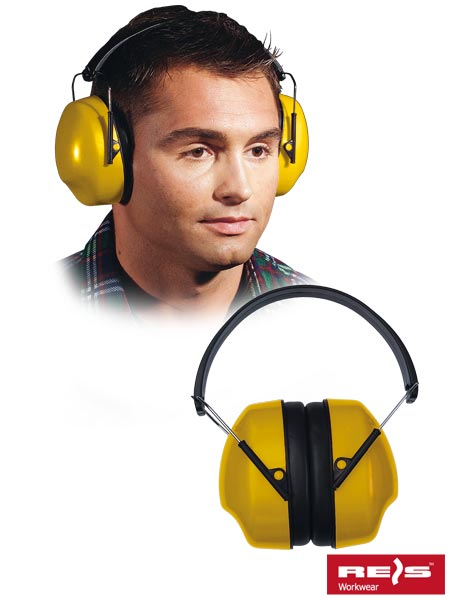
\includegraphics[scale=0.4]{../Assets/nauszniki_bhp.png}
	\caption{Użyte w~projekcie nauszniki ochronne.\\ Źródło: Copyright \textsuperscript{\textcopyright} by REIS GROUP}
	\label{fig:nauszniki_bhp}
\end{figure}

Nauszniki te stanowią część tłumiącą pasywnie. Do stworzenia i~zaimplementowania części aktywnej układu zastosowano wymienione poniżej elektroniczne elementy analogowe oraz cyfrowe, przy czym elementy cyfrowe są wymienione każdy z~osobna, pomimo iż stanowią integralne podzespoły mikrokontrolera.
\begin{enumerate}
	\item Analogowe:
	\begin{itemize}
		\item Pojemnościowy mikrofon elektretowy typu CMA-4544PF-W (rys. \ref{fig:mikrofony_max4466}) -- dwie sztuki\\
		W~urządzeniu zamontowano jeden główny (feedforward) na zewnątrz muszli oraz jeden odsłuchowy (feedback) wewnątrz muszli słuchawki.
		\item Przedwzmacniacz mikrofonowy typu Adafruit MAX4466 -- dwie sztuki\\
		\begin{figure}[h!]
			\centering
			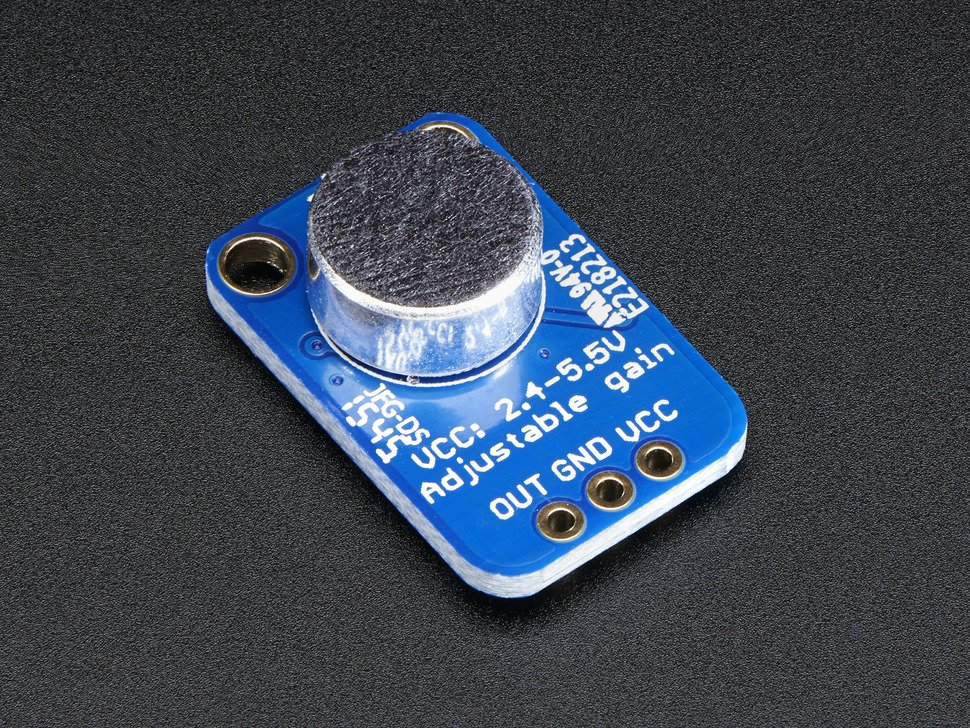
\includegraphics[scale=0.2]{../Assets/adafruit_max4466.png}
			\caption{Użyte w~projekcie mikrofony z~przedwzmacniaczami.\\ Źródło: https://cdn-shop.adafruit.com/970x728/1063-03.jpg}
			\label{fig:mikrofony_max4466}
		\end{figure}
		Wzmacniacz operacyjny zoptymalizowany przez producenta pod kątem wykorzystania z~mikrofonami. Autor zakupił przedwzmacniacz połączony przez producenta z~wyżej wymienionym mikrofonem w~ramach jednej płytki (rys. \ref{fig:mikrofony_max4466}). Należy pamiętać o~przesunięciu fazy sygnału -- jednak ten problem powinien zostać rozwiązany przez filtr adaptacyjny.
		\item Wzmacniacz audio klasy D typu Adafruit PAM8302 (rys. \ref{fig:pam8302})\\
		\begin{figure}[h!]
			\centering
			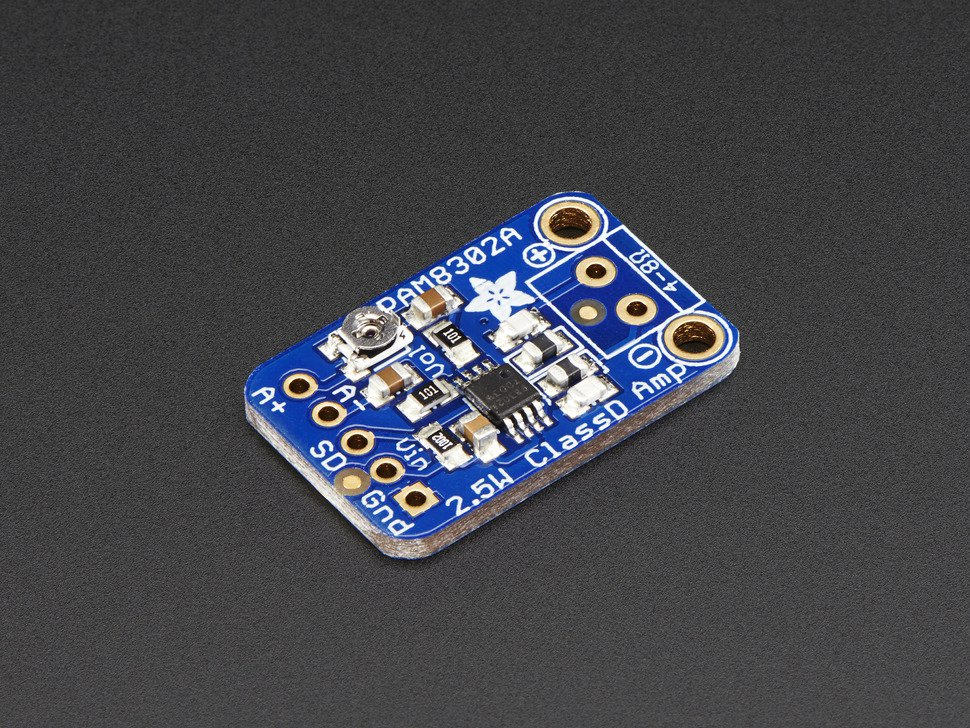
\includegraphics[scale=0.2]{../Assets/wzmacniacz_pam8302.png}
			\caption{Użyty w~projekcie wzmacniacz audio.\\ Źródło: https://cdn-shop.adafruit.com/970x728/2130-01.jpg}
			\label{fig:pam8302}
		\end{figure}
		Ten wzmacniacz monofoniczny o~mocy \SI{2.5}{\W} przeznaczony jest do współpracy z~głośnikami o~impedancji od \SI{4}{} do \SI{8}{\ohm}. Producent deklaruje sprawność w~zakresie 85-88\% \cite{speakeropamp} oraz współczynnik zawartości harmonicznych i~szumów (THD+N) wynoszący 10\%.
		\item Głośnik typu MG15 o~mocy \SI{0.1}{\W} oraz impedancji \SI{8}{\ohm} (rys. \ref{fig:mg15})\\
		\begin{figure}[h!]
			\centering
			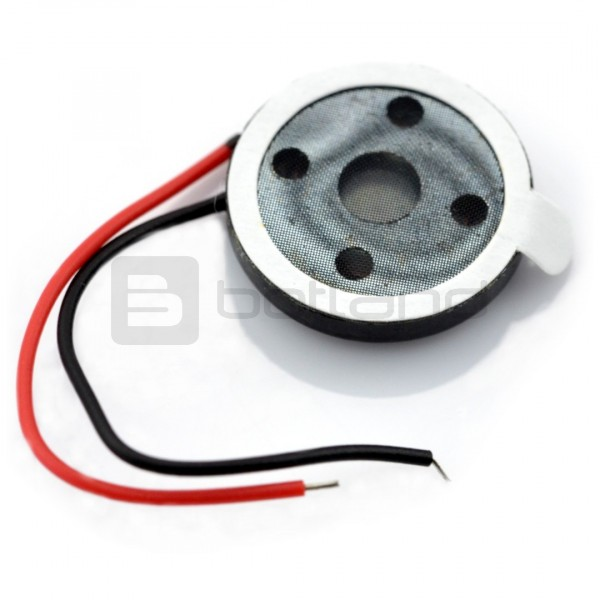
\includegraphics[scale=0.1]{../Assets/glosnik_mg15.png}
			\caption{Użyty w~projekcie głośnik.\\ Źródło: https://botland.com.pl/49567-thickbox\_default/glosnik-mg15-01w-8ohm-15x4mm.jpg}
			\label{fig:mg15}
		\end{figure}
		\item Filtr dolnoprzepustowy (antyaliasingowy) -- dwie sztuki\\
		Zanim sygnał zostanie dostarczony do przetwornika A/C, należy zapewnić, by jego częstotliwość nie przekroczyła częstotliwości Nyquista\footnote{Jest to połowa częstotliwości próbkowania sygnału. Przekroczenie jej przez nieodfiltrowany sygnał powoduje pokrycie się dwóch, różnych od siebie sygnałów. Przykład aliasingu: Dla częstotliwości Nyquista równej \SI{1000}{\Hz}, nieodfiltrowany sygnał \SI{3100}{\Hz} zostałby odczytany jako sygnał \SI{100}{\Hz}.}. Pozwala to uniknąć błędnego zakodowania sygnału w~dziedzinie cyfrowej. W~pracy zastosowano pasywny filtr dolnoprzepustowy RC pierwszego rzędu.
		%\item Filtr dolnoprzepustowy 2 (rekonstrukcyjny, anti-imagingowy)\\
		%Podobnie jak na wejściu do części cyfrowej układu, również na jej wyjściu należy umieścić filtr dolnoprzepustowy (na wyjściu przetwornika C/A) -- aby zapobiec wtłaczaniu wyższych harmonicznych do głośnika.
	\end{itemize}
	\item Cyfrowe:
	\begin{itemize}
		\item Przetwornik analogowo-cyfrowy -- dwie sztuki\\
		Autor zdecydował się użyć dwóch osobnych przetworników (wchodzących w~skład mikrokontrolera) do akwizycji sygnału z~mikrofonów, aby uniknąć przesłuchów, które mogłyby się pojawić w~przypadku użycia pojedynczego przetwornika. Przyczyną przesłuchów jest zwykle multiplekser analogowy wybierający kanały wejściowe przetwornika A/C. Takie rozwiązanie zmniejsza też nieznacznie opóźnienia w~przetworzeniu sygnału, gdyż można wtedy skonfigurować przetworniki w~trybie mierzenia pojedynczego kanału, a~nie skanowania dwóch po kolei. Przetwornik realizuje algorytm SAR\footnote{Sukcesywna Aproksymacja (ang. Successive Approximation Register, inaczej próbkowanie bitowe)}.\\
		Warto zauważyć, że przetworniki dostępne na płytce użytej przez autora mają rozdzielczość 12~bitów, co pozostawia pewne pole do poprawy projektu i~wyboru komponentów, ale jednocześnie zapewnia wystarczający poziom dokładności dla potrzeb prototypowania układu.
		\item Timer (Licznik)\\
		Do zadania wyznaczenia stałego kroku próbkowania wybrano timer~3. Jest to podstawowy licznik mikrokontrolera, bez dodatkowych funkcjonalności (jakie posiada chociażby timer~1). Odmierzenie zadanego interwału czasowego sygnalizowane jest wewnętrznie jako zdarzenie, które wychwytuje przetwornik A/C. Jego konfiguracja została opisana w~sekcji~\ref{sec:configuration}.
		\item Kontroler DMA (Direct Memory Access) -- dwie sztuki\\
		Jeden z~kontrolerów użyty jest do transferu danych z~przetworników~A/C do pamięci mikrokontrolera STM32, zaś drugi - do transferu (po przeprowadzeniu eksperymentu) wartości nastaw filtra LMS z~pamięci do kontrolera UART. Transfer w~pierwszym przypadku dokonywany jest w~trybie ciągłym, a~więc po każdym przerwaniu do DMA, zgłoszonym przez przetwornik na końcu konwersji. W~drugim przypadku, transfer wywoływany jest po wciśnięciu przez testera przycisku na płytce prototypowej lub wysłaniu odpowiedniej komendy z~komputera~PC.
		\item NVIC (Nested Vectored Interrupt Controller)\\
		Kontroler przerwań (zagnieżdżonych), który przyspiesza ich obsługę.
		\item USART (Universal Synchronous/Asynchronous Receiver/Transmitter)\\
		Komponent odpowiedzialny za transmisję danych w~trybie full-duplex pomiędzy mikrokontrolerem a~dowolnym innym urządzeniem obsługującym protokół komunikacji USART. Połączenie UART z~komputerem nie wymagało użycia konwertera USB-UART, gdyż programator/debugger ST-Link, obecny na użytej płytce NUCLEO, posiada podłączone wyprowadzenia UART z~mikrokontrolera. Dane odebrane przez programator są bezpośrednio przekazywane do kontrolera USB, który już jest podłączony do komputera PC. Zatem przy użyciu jednego połączenia można zarówno zasilać urządzenie, programować je, debuggować, jak i~również odbierać z~niego dane.
		\item Rdzeń mikrokontrolera\\
		Główna jednostka obliczeniowa.
		\item FPU (Floating Point Unit)\\
		Jednostka dedykowana do obliczeń zmiennoprzecinkowych na liczbach 32-bitowych (a~więc typu float). Znacznie podnosi precyzję obliczeń na ułamkach i~przyspiesza działanie całego układu jeżeli takich działań jest dużo. Należy jednak pamiętać, że operuje jedynie na danych pojedynczej precyzji. 
		\item Przetwornik cyfrowo-analogowy\\
		Do celu prototypowego użyto jednego kanału wyjściowego, aby przetestować działanie systemu w~jednolitej, odgrodzonej przestrzeni sferycznej. Konwersja sygnału na postać analogową następuje automatycznie, bez oddzielnego inicjowania, przy każdej wykrytej zmianie słowa bitowego wpisanego przez program do rejestru danych wyjściowych przetwornika DAC. Dane są wpisywane do tego rejestru po każdym skończonym cyklu obliczeniowym.
	\end{itemize}
\end{enumerate}

\section{Schemat i konfiguracja układu}
\label{sec:config}
Uproszczony schemat w~wersji graficznej został przedstawiony przez autora na rysunku \ref{fig:schemat1}. Podstawową zasadą działania systemu jest:
\begin{enumerate}
	\item Akwizycja sygnału przez dwa mikrofony: główny oraz odsłuchowy.
	\item Wzmocnienie sygnału przez przedwzmacniacz mikrofonowy.
	\item Konwersja analogowego sygnału do postaci cyfrowej w~przetworniku ADC.
	\item Transfer danych przez kontroler DMA do pamięci urządzenia.
	\item Odczyt danych (pochodzących z~mikrofonu głównego) z~pamięci i~przetworzenie ich w~filtrze FIR.\\
	Odczyt danych (pochodzących z~mikrofonu odsłuchowego) z~pamięci i~przetworzenie ich w~module strojenia LMS.
	\item Jednoczesne przekazanie danych z~mikrofonu głównego do modułu strojenia filtra LMS.
	\item Przestrojenie filtra na podstawie algorytmu LMS.
	\item Obliczenie odpowiedzi filtra FIR i~przesłanie jej do przetwornika DAC.
	\item Wzmocnienie sygnału przez wzmacniacz audio.
	\item Odtworzenie sygnału wytłumiającego przez głośnik.
\end{enumerate}
\begin{figure}[h!]
	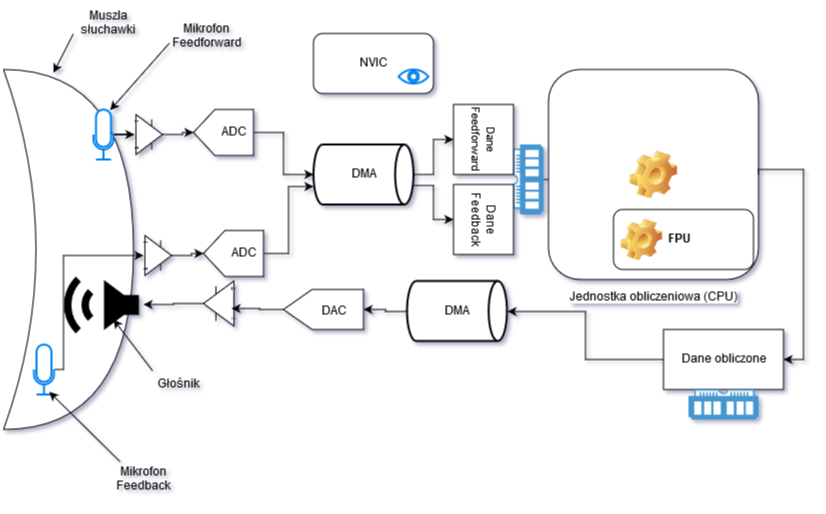
\includegraphics[width=\linewidth]{../Assets/schemat_ukladu.png}	
	\caption{Schemat układu.}
	\label{fig:schemat1}
\end{figure}
Autor pominął pomniejsze elementy, które nie wnoszą szczególnych informacji do opisu pracy. W~kwestii umiejscowienia mikrofonu odsłuchowego autor posłużył się wnioskami przedstawionymi w~artykule dotyczącym aktywnej redukcji hałasu w~zastosowaniach słuchawek tłumiących \cite{ANC4HP}. Autorzy pracy na podstawie widma częstotliwościowego wyznaczyli optymalne położenie mikrofonu i~wykazali, że takim miejscem jest bliskie otoczenie przewodu słuchowego zewnętrznego. Konkretne położenie mikrofonu odsłuchowego ilustruje lokacja nr~8 na rysunku \ref{fig:error_mic_placement} zapożyczonym z~wyżej wymienionej pracy.
Mikrofon odsłuchowy umiejscowiony w~optymalnej pozycji charakteryzuje się zlinearyzowaną odpowiedzią częstotliwościową, co ogranicza błędy pomiarowe, poprawiając precyzję zastosowanego rozwiązania.
\begin{figure}[h!]
	\centering
	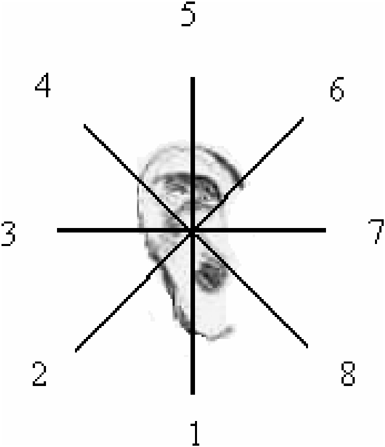
\includegraphics[scale=0.6]{../Assets/error_mic_placement.png}
	\caption{Położenie mikrofonu odsłuchowego odzwierciedla lokacja nr 8.\\ Źródło: \fullcite{ANC4HP}; strona 333}
	\label{fig:error_mic_placement}
\end{figure}

Aby stworzyć odgrodzoną przestrzeń sferyczną, autor postanowił złączyć (ścisnąć) dwie słuchawki użytych nauszników. Pomiędzy słuchawkami umieszczono element dystansowy (długopis), aby zamodelować nieidealne przyleganie słuchawek do głowy potencjalnego użytkownika. Do celów testowych nie będzie potrzebny dodatkowy mikrofon umieszczony w~środku przestrzeni -- zostanie użyty zamontowany już mikrofon odsłuchowy. Dane z~niego zostaną odczytane przy użyciu sondy oscyloskopu.

Aby zasilić prototyp, autor podłączył mikrokontroler poprzez USB do komputera osobistego. Zapewniło to standardowe zasilanie mikrokontrolera na poziomie \SI{3.3}{\V}. Ponadto, celem odseparowania części analogowej od cyfrowej, autor zdecydował się zapewnić osobne zasilanie dla układów analogowych, a~więc mikrofonu wraz z~jego przedwzmacniaczem oraz dla wzmacniacza głośnikowego. Tym samym zredukowane są zakłócenia, które normalnie mogłyby się przenieść z~linii zasilania układu cyfrowego do bardzo wrażliwej na te zakłócenia części analogowej. Zasilanie to, dla mikrofonów, zostało osiągnięte poprzez dołączenie pastylkowych baterii \SI{3}{\V} typu CR2032 do elementów analogowych. Zasilanie przedwzmacniacza z~głośnikiem wymaga użycia nieco innej metody ze względu na dużą moc komponentu -- zwykła bateria nie wystarczyłaby do odpowiednio długotrwałego działania układu. Biorąc pod uwagę prototypowy charakter całego urządzenia oraz konieczność połączenia mikrokontrolera z~komputerem, autor zdecydował się zasilić przedwzmacniacz przy użyciu modułu zasilającego z~płytki stykowej, podłączonego przez zasilacz impulsowy DC \SI{9}{\V} do gniazdka sieciowego. Przyłącze zasilacza nie posiada złącza uziemienia, dlatego po połączeniu wszystkich komponentów w~całym układzie występuje jeden wspólny punkt uziemiający -- jest nim GNDA, czyli masa analogowa mikrokontrolera. Pozwala to uniknąć pętli masy, które miałyby wpływ na jakość sygnału w~urządzeniu. Warto zwrócić uwagę na fakt, że gdyby zasilający wzmacniacz mocy został podłączony przez magistralę USB, to powstałaby pętla masy pomiędzy układem mierzonym a~komputerem pomiarowym, który zasila już zestaw uruchomieniowy z~mikrokontrolerem.
\chapter{Hardware -- konfiguracja}

\section{Obliczeniowa platforma sprzętowa}

\section{Konfiguracja peryferiów}


\chapter{Software -- implementacja}
\label{cha:software}
W~tym rozdziale autor przedstawia sposób, w~jaki zaprogramowany został system. Uwzględnione oraz pokazane są tutaj różnice między typowym algorytmem FIR+LMS wspomnianym w~sekcji \ref{FIRLMS} rozdziału \ref{cha:teoria}, a~zaproponowanym przez autora wariantem rozwiązania i~charakterystycznym dla niego sposobem przetwarzania danych.
 
\section{Schemat przetwarzania danych}
Schemat rozwiązania autora jest niemalże równoważny schematowi typowego algorytmu, różni się jednak kolejnością i~charakterem pewnych działań. Podczas gdy we~wspomnianym wcześniej wariancie błąd obliczany/mierzony jest na podstawie sygnału wyjściowego, tworzonego z~kolei na podstawie sygnału wejściowego oraz wartości współczynników w~danej chwili czasu, to w~wersji zaprojektowanej przez autora pomiar błędu następuje w~tej samej chwili, co pomiar sygnału wejściowego. Oznacza to zatem, że należy nieco zmienić kolejność wykonywanych czynności, co ukazuje poniższa tabela.
\begin{table}[h]
	\centering
	\caption{Porównanie schematów przetwarzania danych dla wspomnianego wcześniej algorytmu oraz wersji użytej przez autora.}
	\begin{tabular}{|p{.45\textwidth}|p{.45\textwidth}|}
		\toprule Klasyczny algorytm filtracji & Implementacja autora \\ \midrule
		\begin{enumerate}	
			\item Odczyt sygnału wejściowego x(n).
			\item Obliczenie sygnału wyjściowego y(n).
			\item Odczyt sygnału odsłuchowego e(n).
			\item Aktualizacja wartości współczynników filtra w(n).
		\end{enumerate} & 
		\begin{enumerate}	
			\item Odczyt sygnału wejściowego x(n) oraz sygnału odsłuchowego e(n).
			\item Aktualizacja wartości współczynników filtra w(n).
			\item Obliczenie sygnału wyjściowego y(n).
		\end{enumerate}\\ \bottomrule
	\end{tabular}
\end{table}

Kluczowe jest zatem zrozumienie, że w~n-tej chwili czasu mierzona jest wartość sygnału odsłuchowego odpowiadająca wartościom z~poprzedniej chwili czasu. Dlatego więc należy zaraz po odczytaniu zaktualizować wagi filtra, by zawsze obliczać sygnał wyjściowy na podstawie aktualnych danych.
\section{Implementacja algorytmu}
Algorytm został zaprogramowany w~języku~C przy użyciu środowiska System Workbench for STM32. Użyty typ zmiennych realizujących obliczenia to liczby zmiennoprzecinkowe pojedynczej precyzji ''float''. Aby skorzystać ze zwiększonej dokładności, jaką daje ten typ zmiennej, autor skonwertował zmienną przechowującą słowo bitowe (wynik pomiaru przetwornika) z~typu stałoprzecinkowego na zmiennoprzecinkowy, stosując w~pewnym sensie odwrócenie konwersji przetwornika. Słowo bitowe zostało przekonwertowane na poziom napięcia, od którego następnie odjęto $ \frac{V_{ref}}{2} $, aby z~sygnału usunąć składową stałą. Jest to działanie konieczne dla poprawnego wykonywania operacji zgodnych z~algorytmem filtra. Po aktualizacji wag oraz obliczeniu sygnału wyjściowego, z powrotem dokonywana jest konwersja do słowa bitowego. Można więc powiedzieć, że programowo realizowany jest dodatkowy tor przetwarzania sygnału z~cyfrowego na pseudoanalogowy i~odwrotnie. Straty dokładności pochodzące z~tej zaprogramowanej konwersji są jednak znacznie mniejsze w~porównaniu do strat i~nakładu pracy pochodzącej z~wykonywania tych samych operacji na liczbach stałoprzecinkowych.

Miejsce wykonania algorytmu umieszczono w~funkcji obsługującej przerwanie pochodzące od kontrolera DMA, informujące o~skończonym transferze danych z~obu przetworników~ADC.
\section{Dobór nastaw algorytmu}
\chapter{Walidacja rozwiązania}
\label{cha:tests}
Po wstępnym nastrojeniu układu, należy uruchomić oraz przetestować urządzenie. Autor zapoznał się w~tym celu z~normą dotyczącą mierzenia poziomu natężenia hałasu \cite{test_norm}, jednak ze względów subiektywnych zastosował się jedynie do zaleceń traktujących o~metodzie pomiarowej, nie zaś do dokładnego sposobu wykonania pomiaru. Zarówno sposób, jak i~wyniki pomiarów, opisane są w~sekcji \ref{sec:practical_test}.
\section{Test praktyczny}
\label{sec:practical_test}
Celem sprawdzenia jakości zbudowanego urządzenia, autor dokonał testu praktycznego, w~którym zmierzył poziom natężenia dźwięku w~pewnym pomieszczeniu ze stałym, powtarzalnym typem hałasu, w~trzech wariantach -- bez tłumienia, tylko z~tłumieniem pasywnym, oraz z~tłumieniem pasywnym i~uruchomionym tłumieniem aktywnym pochodzącym z~zaprogramowanego układu.
\subsection{Warunki testu}
\label{subsec:circumstances}
Układ został przetestowany w~pomieszczeniu monitoringowym przeznaczonym dla ochrony biurowca. Pomieszczenie jest niewielkie i~znajduje się w~nim wiele urządzeń elektrycznych -- komputery, monitory, wiatraki, zasilacze oraz szafka z~urządzeniami sieciowymi, których układy chłodzące generują dość uciążliwy przy długotrwałej ekspozycji hałas. Pokój, który wykorzystano do testów, znajduje się na uboczu budynku, z~dala od pomieszczeń biurowych, gdzie znajdują się pracownicy. Pozwala to zatem na przetestowanie działania układu przy powtarzalnym hałasie o~niskiej częstotliwości. Pewne dźwięki oczywiście mimo wszystko przedostaną się do pokoju, nie będą jednak głównym elementem składowym danego typu hałasu mierzonego w~tym pomieszczeniu. Urządzenie umieszczono w~środku pomieszczenia i~skierowano je mikrofonem w~stronę szafki z~urządzeniami sieciowymi, które w~tym teście są głównym źródłem hałasu. Odległość od źródła dźwięku wynosiła PLACEHOLDER, %TODO ILE METRÓW???? 
zaś czas pomiaru wynosił 15~sekund dla każdego z~etapów.
\subsection{Typowe rodzaje hałasu}
Jak już wspomniano w~sekcji \ref{sec:hałas} rozdziału \ref{cha:teoria}, typowymi rodzajami hałasu, które można chcieć tłumić takim urządzeniem, są:
\begin{itemize}
	\item rozmowy pobliskich osób,
	\item szum wentylacyjny,
	\item dźwięk towarzyszący pracy silnika.
\end{itemize}
Są to zatem sygnały charakteryzujące się (w~przybliżeniu) stałym przedziałem częstotliwościowym i~niewielkim natężeniem, jednak będące uciążliwymi w~dłuższej perspektywie czasowej. W~ramach testu praktycznego sprawdzono działanie układu przy ekspozycji na hałas pochodzący od rozmowy kilku osób w~biurze oraz na szum wentylatorów i~pobliskich urządzeń elektrycznych.
\subsection{Poziom hałasu bez tłumienia}
Pomiaru bez tłumienia dokonano przy otwartej muszli słuchawek i~wyłączonym algorytmie. Zbierano dane z~mikrofonu odsłuchowego (feedback). Pozwoliło to na zebranie danych o~poziomie natężenia hałasu w~miejscu, w~którym znajdowało się urządzenie. Przy założeniu opisanych w~sekcji \ref{subsec:circumstances} warunków testu, średni poziom hałasu zmierzony bez żadnego sposobu tłumienia wyniósł PLACEHOLDER. %TODO uzupełnić pomiar.
Widmo częstotliwościowe pokazano na rysunku \ref{fig:widmo_bez}.
\begin{figure}[h!]
	\centering
	\includegraphics{../Assets/widmo_bez_tlumienia.png}
	\caption{Widmo częstotliwościowe hałasu przy pomiarze bez tłumienia hałasu.}
	\label{fig:widmo_bez}
\end{figure}

\subsection{Poziom hałasu z pasywnym tłumieniem}
Następnie, aby dokonać pomiaru natężenia hałasu przy pasywnym tłumieniu, zamknięto i~zebrano dane pochodzące z~drugiego mikrofonu (feedback). Dzięki temu otrzymano informację o~tym, jaki poziom hałasu panuje wewnątrz słuchawki, czyli jaki hałas słyszałby użytkownik przy użyciu jedynie pasywnego tłumienia, które dają użyte nauszniki. Przy tych samych założeniach, średni poziom hałasu wyniósł PLACEHOLDER2. %TODO uzupełnić pomiar.
Widmo częstotliwościowe zaprezentowano na rysunku \ref{fig:widmo_pasywnie}. 
\begin{figure}[h!]
	\centering
	\includegraphics{../Assets/widmo_pasywnie.png}	
	\caption{Widmo częstotliwościowe hałasu przy pomiarze z~pasywnym tłumieniem.}
	\label{fig:widmo_pasywnie}
\end{figure}

\subsection{Poziom hałasu z aktywnym tłumieniem}
Ostatecznie, aby dowieść skuteczności rozwiązania, uruchomiono algorytm i~ponownie zebrano dane z~mikrofonu odsłuchowego. Średni poziom hałasu zmierzony w~ten sposób wyniósł PLACEHOLDER3. %TODO uzupełnić pomiar.
Widmo częstotliwościowe zamieszczono na rysunku \ref{fig:widmo_aktywnie}.
\begin{figure}[h!]
	\centering
	\includegraphics{../Assets/widmo_aktywnie.png}	
	\caption{Widmo częstotliwościowe hałasu przy pomiarze z~aktywnym tłumieniem.}
	\label{fig:widmo_aktywnie}
\end{figure}

Dodatkowo, aby porównać zbudowany układ do istniejącego rozwiązania rynkowego, ten sam pomiar wykonano dla słuchawek Jabra Elite~80. Tak jak urządzenie autora, używają one podejścia feedforward-feedback.\cite{JabraEvolve80} Sposób realizacji rozwiązania (analogowy czy cyfrowy) nie jest nigdzie wyjawiony, można jednak domniemywać użycie analogowego toru tłumienia ze względu na dużo niższe zużycie energii elektrycznej oraz wymiary takiego układu. Słuchawki podłączono do komputera osobistego i~umieszczono w~tym samym miejscu, w~którym wcześniej mierzono urządzenie autora. Sygnał z~wnętrza słuchawek zbierano poprzez włożenie do muszli słuchawek komercyjnych mikrofonu odsłuchowego z~urządzenia autora (wciąż podpiętego do mikrokontrolera) i~przesłanie danych z~niego (za pośrednictwem modułu komunikacji UART) do komputera monitorującego test. Średni poziom hałasu wewnątrz słuchawek firmowych zmierzony w~ten sposób wyniósł PLACEHOLDER4. Widmo częstotliwościowe tak zmierzonego dźwięku pokazano na rysunku \ref{fig:widmo_jabra}.
\begin{figure}[h!]
	\centering
	\includegraphics{../Assets/widmo_jabra.png}	
	\caption{Widmo częstotliwościowe hałasu przy pomiarze z~aktywnym tłumieniem słuchawek komercyjnych Jabra Elite~80.}
	\label{fig:widmo_jabra}
\end{figure}
%TODO mikrofon z peceta do przestrzeni, zmierzyc widmo dzwieku do matlaba
\chapter{Podsumowanie i wnioski}
\label{cha:wnioski}
W~tym rozdziale autor podsumowuje wyniki pomiarów z~poprzedniego rozdziału, ocenia jakość rozwiązania względem istniejącego rozwiązania komercyjnego oraz proponuje możliwe usprawnienia swojego projektu.
\section{Ocena jakości rozwiązania}
Koszt zbudowanego urządzenia, po podliczeniu kosztów wszystkich komponentów zamówionych w~sklepie internetowym Botland, oraz kosztu nauszników ochronnych, zamyka się w~granicach~230~zł. Poszczególne elementy składające się na tę kwotę znajdują się w~tabeli \ref{tab:costs}.
\begin{table}[h!]
	\centering
	\caption{Wyliczenie kosztów poszczególnych elementów składowych projektu.}
	\label{tab:costs}
		\begin{tabular}{|p{.30\textwidth}|p{.30\textwidth}|p{.20\textwidth}|}
		\toprule Element & Opis & Koszt \\ \midrule
		\begin{enumerate}	
			\item NUCLEO-F446RE
			\item 2x Adafruit MAX4466
			\item Adafruit PAM8302
			\item Głośnik MG15
			\item Nauszniki ochronne
			\item Zestaw płytka stykowa + przewody + moduł zasilający
		\end{enumerate} & 
		\begin{enumerate}	
			\item Płytka prototypowa z~mikrokontrolerem.
			\item Mikrofon elektretowy ze wzmacniaczem audio.
			\item Przedwzmacniacz audio dedykowany do głośników.
			\item Głośnik \SI{0,1}{\W} o~impedancji \SI{8}{\Omega}
			\item Typowe, tanie nauszniki ochronne ze sklepu BHP.
			\item Podstawowy zestaw płytki stykowej 830 pól, przewody oraz moduł zasilający MB102.
		\end{enumerate} &
		\begin{enumerate}
			\item 77,90 zł
			\item 79,80 zł
			\item 19,90 zł
			\item 2,20 zł
			\item 22,50 zł
			\item 19,90 zł
		\end{enumerate}\\ \bottomrule
	\end{tabular}
\end{table}

Zatem sumaryczny koszt takiego rozwiązania wynosi, według tabeli \ref{tab:costs}, 222,20 zł. Należy pamiętać, że jest to kwota brutto za zamówienie małej liczby elementów -- przy zamówieniu hurtowym części do masowej produkcji urządzenia, cena byłaby dużo niższa.

W~porównaniu do słuchawek Jabra Elite 80, które można kupić w~cenie wahającej się między 1000~zł, a~1400~zł\footnote{Wyniki wyszukiwania serwisu ceneo.pl, stan z~dnia 04.01.2020.}, jest to dobra cena, jeśli weźmie się pod uwagę fakt, że dokupienie dodatkowych elementów i~zmodyfikowanie układu tak, by spełniał funkcję słuchawek, nie zwiększy jego ceny nawet dwukrotnie.

TUTAJ WNIOSKI DALSZE I OCENA JAK TO W OGOLE DZIALA
\section{Propozycja możliwych usprawnień}
Biorąc pod uwagę decyzje konstrukcyjne, ograniczenia użytej platformy oraz wyniki testów, autor proponuje następujące usprawnienia swojego projektu:
\begin{enumerate}
	\item Użycie dedykowanej płytki z~mikrokontrolerem, zamiast płytki prototypowej, która zawiera niepotrzebne w~tym układzie elementy.\\
	Pozwoliłoby to na obniżenie kosztów jednostki centralnej i~zmniejszenie wymiarów urządzenia -- przy użyciu dedykowanej płytki, można by od razu wytrawić na niej połączenia, które w~obecnym stanie łączone są poprzez płytkę stykową.
	\item Dokładniejsze zamocowanie elementów w~słuchawce.\\
	Obecnie, mikrofon główny, odsłuchowy i~głośnik połączone są dość luźno z~nausznikami. Urządzenie działałoby na pewno sprawniej, gdyby przytwierdzono te elementy na stałe i~dostosowano ich rozmiar oraz otoczenie do współpracy, gdyż w~tym momencie są to niezwiązane ze sobą części, połączone do celów prototypowych.
	\item Rozszerzenie funkcjonalności urządzenia o~drugi kanał.\\
	Dodanie kanału stereo, drugiego głośnika i~drugiego mikrofonu odsłuchowego pozwoliłoby na pełnoprawne korzystanie z~nauszników -- w~tym momencie jest to jedynie odgrodzona sferyczna przestrzeń, którą tworzą dwie złączone słuchawki.
	\item Dodanie możliwości słuchania pożądanego sygnału w~urządzeniu.\\
	Urządzenie obecnie jedynie tłumi sygnał -- mogłoby jednak tłumić i~jednocześnie odtwarzać muzykę lub inne pożądane dźwięki, tak jak robią to słuchawki komercyjne stosowane na rynku.
	\item Ujednolicenie zasilania.\\
	W~tym momencie cały system zasilany jest z~trzech punktów:
	\begin{itemize}
	\item Zasilanie USB przypięte do płytki prototypowej NUCLEO-F446RE,
	\item Zasilanie USB przypięte do modułu zasilającego przedwzmacniacz audio,
	\item Zasilanie bateryjne dostarczające energię do mikrofonów urządzenia.
	\end{itemize}
	Ograniczenie liczby podpięć układu do jednego ułatwiłoby używanie urządzenia i~zwiększyłoby jego mobilność.
\end{enumerate}

Powyższe propozycje są jedynie przykładowymi sposobami ulepszenia działania lub dodania nowych funkcjonalności urządzenia.
\section{Wnioski ogólne}
Prototypowanie urządzeń przy użyciu mikrokontrolerów STM32 jest prostsze względem projektowania układów analogowych lub cyfrowych nieużywających tego typu mikrokontrolera. Zapewnia to mnogość dokumentacji i~narzędzi dostarczanych na bieżąco przez producentów oprogramowania.

Bardzo często wykorzystuje się mikrokontrolery do zaprojektowania i~przetestowania układu, który później zostaje wykonany w~wersji analogowej dla zaoszczędzenia energii i~zmniejszenia wymiarów ostatecznej postaci urządzenia.


i tak dalej i tak dalej i żyli długo i szczęśliwie za siedmioma sinusami


% itd.
% \appendix
% \include{dodatekA}
% \include{dodatekB}
% itd.

\printbibliography

\end{document}
